% ============================================================
%  IEEE Transactions — Kill-Chain MaxSAT Honeypot Placement
%  v7 — Extended Related Work + Cross-Path + Six-Objective
%       Deep Analysis + Missing Critical Citations ADDED
% ============================================================
\documentclass[journal]{IEEEtran}

\usepackage{amsmath,amssymb,amsfonts}
\usepackage{amsthm}
\usepackage{algorithmic}
\usepackage{algorithm}
\usepackage{array}
\usepackage{graphicx}
\usepackage{textcomp}
\usepackage[table]{xcolor}
\usepackage{booktabs}
\usepackage{multirow}
\usepackage{url}
\usepackage{hyperref}
\usepackage{cite}
\usepackage{balance}
\usepackage{pifont}
\usepackage{mdframed}
\usepackage{subcaption}
\usepackage{rotating}
\usepackage{tikz}
\usetikzlibrary{matrix,positioning,fit,backgrounds,
                decorations.pathreplacing,arrows.meta}

\hypersetup{colorlinks=true,linkcolor=blue,
            citecolor=blue,urlcolor=blue}

% ── theorem environments ─────────────────────────────────────
\newtheorem{theorem}{Theorem}
\newtheorem{lemma}[theorem]{Lemma}
\newtheorem{definition}[theorem]{Definition}

% ── check/cross marks ────────────────────────────────────────
\newcommand{\cmark}{\textcolor{novelgreen}{\ding{51}}}
\newcommand{\xmark}{\textcolor{novelred}{\ding{55}}}
\newcommand{\pmark}{\textcolor{novelamber}{\textbf{\textasciitilde}}}

% ── novelty-gap colours ──────────────────────────────────────
\definecolor{novelgreen}{RGB}{0,130,70}
\definecolor{novelred}{RGB}{185,30,30}
\definecolor{novelamber}{RGB}{195,120,0}
\definecolor{hdrblue}{RGB}{25,70,140}
\definecolor{rowours}{RGB}{210,240,220}
\definecolor{cellck}{RGB}{215,240,220}
\definecolor{cellxk}{RGB}{245,210,210}
\definecolor{cellpk}{RGB}{250,235,195}

% ── proof highlight box ──────────────────────────────────────
\definecolor{proofbg}{RGB}{245,250,255}
\definecolor{proofborder}{RGB}{30,80,160}
\newmdenv[
  backgroundcolor=proofbg,
  linecolor=proofborder,
  linewidth=1.5pt,
  leftmargin=0pt, rightmargin=0pt,
  innerleftmargin=8pt, innerrightmargin=8pt,
  innertopmargin=6pt, innerbottommargin=6pt
]{proofbox}

% ── insight box (green) ──────────────────────────────────────
\definecolor{insightbg}{RGB}{240,252,240}
\definecolor{insightborder}{RGB}{0,130,70}
\newmdenv[
  backgroundcolor=insightbg,
  linecolor=insightborder,
  linewidth=1.5pt,
  leftmargin=2pt, rightmargin=2pt,
  innerleftmargin=6pt, innerrightmargin=6pt,
  innertopmargin=5pt, innerbottommargin=5pt
]{insightbox}

% ── coloured example boxes ───────────────────────────────────
\definecolor{exbg}{RGB}{240,248,255}
\definecolor{exborder}{RGB}{0,102,204}
\newmdenv[
  backgroundcolor=exbg,
  linecolor=exborder,
  linewidth=1.5pt,
  leftmargin=2pt, rightmargin=2pt,
  innerleftmargin=5pt, innerrightmargin=5pt,
  innertopmargin=4pt, innerbottommargin=4pt
]{examplebox}

% ── macros ───────────────────────────────────────────────────
\newcommand{\ie}{\emph{i.e.}}
\newcommand{\eg}{\emph{e.g.}}
\newcommand{\etal}{\emph{et~al.}}
\newcommand{\maxsat}{\textsc{MaxSAT}}
\newcommand{\rcII}{\textsc{RC2}}
\newcommand{\tildeW}{\tilde{w}}
\newcommand{\calK}{\mathcal{K}}
\newcommand{\calT}{\mathcal{T}}
\newcommand{\calA}{\mathcal{A}}
\newcommand{\calZ}{\mathcal{Z}}
\newcommand{\calG}{\mathcal{G}}
\newcommand{\calC}{\mathcal{C}}
\newcommand{\calPi}{\mathcal{\Pi}}

% ============================================================
\begin{document}

\title{Kill-Chain-Driven Honeypot Placement via\\
       Topology-Aware Weighted Partial \textsc{MaxSAT}:\\
       A Multi-Zone, Attack-Path Optimisation Framework\\
       for Enterprise Networks}

\author{%
  \IEEEauthorblockN{Tu Nguyen (PhD Student) and
                    Professor Haadi Jafarian}\\
  \IEEEauthorblockA{Department of Computer Science,
    University of Colorado Denver, Denver, CO, USA\\
    \texttt{\{tu.nguyen, haadi.jafarian\}@ucdenver.edu}}%
}

\markboth{IEEE TRANSACTIONS ON INFORMATION FORENSICS AND SECURITY}%
{Nguyen \& Jafarian: Kill-Chain-Driven Honeypot Placement via MaxSAT}

\maketitle

% ============================================================
\begin{abstract}
Deciding where to place honeypots in a large company network
is surprisingly hard.
The network is split into different security zones, contains
thousands of different types of servers, and faces attackers
who follow well-known step-by-step attack patterns called
kill chains.
On top of that, the organisation has a limited budget, and
some honeypot types cannot be deployed at the same time
because they would conflict with each other.

In this paper, we model honeypot placement as a
\textbf{Weighted Partial Maximum Satisfiability (\maxsat{})}
problem.
We encode six goals at once: how well we detect threats,
how many attack techniques we cover from the MITRE ATT\&CK
framework, how many attack tactic families we cover, how well
we stop attackers early, how well we catch attackers at the
end of their path, and how good our coverage is across all
attack paths.
All hard rules---budget limits, zone isolation, and conflict
constraints---are encoded as clauses that must never be
violated.
We formally prove that the honeypot placement decision
problem is NP-hard, justifying why a complete solver like
RC2 is necessary over any greedy heuristic.

We test our approach on networks ranging from 100 nodes
(tiny) to over 5.5 million nodes (very large), simulating
five different real-world attack scenarios.
Our \maxsat{} solver achieves a quality score of $Q=67.4$
compared to $Q=52.8$ for the best competing approach
($+27.8\%$), while also providing a mathematical guarantee
that its answer is the best possible solution.
\end{abstract}

\begin{IEEEkeywords}
Honeypot placement, Weighted Partial MaxSAT, kill chain,
MITRE ATT\&CK, network deception, multi-zone topology,
NP-hardness, proactive cyber defence, RC2 solver, enterprise
network security.
\end{IEEEkeywords}

% ============================================================
\section{Introduction}
\label{sec:intro}
% ============================================================

\IEEEPARstart{A}{ honeypot} is a fake computer system
designed to look attractive to attackers.
When an attacker interacts with it, the defender learns about
their methods and can raise an alert.
Honeypots are widely used in network security, but their
usefulness depends heavily on \emph{where} they are placed.
If a honeypot is put in the wrong place, it will never be
visited by attackers and the investment is wasted.

Real company networks make this placement decision much
harder than it sounds.
Consider a typical large organisation.
It has an internet-facing area (called a DMZ) where its
public web servers sit.
It has an internal office network.
It might have cloud services.
It may also have industrial control systems (called OT/SCADA)
that run physical equipment like power plants or factories.
Each of these areas has different security rules, different
types of computers, and different risks.
Attackers do not wander randomly through these areas---they
follow structured plans called kill chains~\cite{hutchins2011},
moving step by step from one zone to another toward their
final target.

The problem is further complicated by three facts.
First, the organisation has a limited budget and cannot afford
to deploy a honeypot on every machine.
Second, certain combinations of honeypot types are
incompatible---for example, an industrial control system
honeypot deployed in the cloud zone would be useless because
the OT zone is physically isolated from the cloud.
Third, there are many possible attack paths through the
network and an ideal placement should intercept as many as
possible.

Existing methods do not handle all these challenges at the
same time.
Simple rule-based approaches just follow fixed guidelines.
Greedy algorithms pick the best-looking option at each step
but cannot reverse a bad decision.
Game-theoretic approaches~\cite{kiekintveld2015,pawlick2019}
model honeypot placement as a strategic interaction but
assume flat networks without zone isolation or budget
conflict constraints.
Reinforcement learning methods~\cite{huang2019} learn how to
\emph{engage} attackers after placement decisions have
already been made, but do not optimise the initial placement
itself.
In this paper, we use a formal solver that considers
\emph{all} constraints and objectives together and provides
a \emph{proven optimal} answer.
We also formally prove that the problem is NP-hard
(Theorem~\ref{thm:nphard}), which means that no
polynomial-time algorithm can always find the optimal
placement---making our complete MAXSAT solver not just a
good choice, but the correct one.

Our main contributions are:
\begin{enumerate}
\item \textbf{A six-goal placement objective} encoded as a
single \maxsat{} optimisation problem comprising:
(1)~detection efficiency,
(2)~coverage of MITRE ATT\&CK attack techniques,
(3)~coverage of MITRE ATT\&CK tactic families,
(4)~catching attackers early in their path,
(5)~catching attackers at the end of their path for forensic
evidence, and
(6)~covering as many attack paths as possible.
Each of these six objectives addresses a different failure
mode of prior methods, and together they create a
solver that is simultaneously prevention-oriented,
intelligence-driven, budget-aware, and topology-correct.

\item \textbf{A formal NP-hardness proof} showing that the
honeypot placement decision problem is NP-hard via
polynomial-time reduction from Weighted Maximum Coverage.
This result formally justifies why a complete solver is
necessary over any greedy or heuristic approach.

\item \textbf{A cross-path force-multiplier encoding} that
lets the solver discover---and exploit---situations where one
honeypot simultaneously satisfies soft clauses across
multiple attack paths, giving a $2.1\times$ advantage over
greedy methods that evaluate only one path at a time.

\item \textbf{A thorough experimental evaluation} across six
different network sizes, using a Monte Carlo simulation to
model attacker behaviour and testing what happens when threat
intelligence updates cause us to re-run the solver with new
priorities.
\end{enumerate}

The rest of this paper is organised as follows.
Section~\ref{sec:related} discusses related work.
Section~\ref{sec:problem} defines the problem formally and
proves NP-hardness.
Section~\ref{sec:formulation} presents our \maxsat{} model.
Section~\ref{sec:methodology} describes our experiments.
Section~\ref{sec:results} presents the results.
Section~\ref{sec:dynamics} explains why our approach beats
the baselines.
Section~\ref{sec:discussion} covers limitations and future
work.
Section~\ref{sec:conclusion} concludes.

% ============================================================
\section{Related Work}
\label{sec:related}
% ============================================================

This section reviews five bodies of research most relevant
to our work: honeypot placement, game-theoretic and
reinforcement-learning-based deception, MITRE ATT\&CK-based
defence, formal methods for network security, and
moving-target defence.
For each body of work we describe what it achieves, explain
its limitations relative to our problem, and identify the
specific gap it leaves.
We then provide a systematic novelty analysis with a
capability matrix (Figure~\ref{fig:novelty_gap}) and an
end-to-end pros-and-cons comparison table
(Table~\ref{tab:proscons}) that maps every baseline against
our approach across all six objectives.

% ------------------------------------------------------------
\subsection{Honeypot Placement Research}

Honeypots have been studied for decades.
Early work focused on making individual honeypots realistic
enough to fool attackers~\cite{spitzner2003}.
Provos built a system that could run many virtual honeypots
on one machine~\cite{provos2004}, which made large-scale
deployment practical.
Spitzner popularised the idea of honeynets---groups of
honeypots that together simulate an entire
network~\cite{spitzner2003}.
However, most of this early work assumed a human expert
would decide where to put the honeypots; there was no
automated decision-making process.

\textbf{Pros:} These works established the foundational
concepts of honeypot realism and honeynet coordination.
\textbf{Cons:} No automated placement, no budget constraints,
no multi-zone topology, and no kill-chain awareness.
They cannot be directly used in a large enterprise network
without substantial manual engineering effort.

% ------------------------------------------------------------
\subsection{Game-Theoretic Honeypot Placement}

Game theory has been the dominant framework for automated
honeypot placement decisions over the past decade.
Kiekintveld \etal{}~\cite{kiekintveld2015} provided one of
the earliest rigorous game-theoretic analyses of honeypot
deployment, modelling the interaction as a Stackelberg game
where the defender commits to a placement strategy and the
attacker responds optimally.
They showed that this formulation leads to mixed-strategy
equilibria that are strictly better than any deterministic
placement.
Yuill \etal{}~\cite{yuill2004} were among the first to frame
deceptive file placement as a strategic interaction.
Tan \etal{}~\cite{tan2011} and Pawlick \etal{}~\cite{pawlick2019}
extended this line of work using formal game theory to model
how rational attackers respond to deception, providing a
comprehensive taxonomy of defensive deception strategies
across six categories including honeypots, obfuscation, and
moving-target techniques.
Wang \etal{}~\cite{wang2018} surveyed this entire landscape,
reviewing over 30 papers on cyber deception and identifying
the key open problems that remain unsolved.

\textbf{Pros:} Game-theoretic methods are mathematically
rigorous. They model rational attacker behaviour explicitly,
produce equilibrium strategies that are provably stable, and
can handle uncertainty in attacker knowledge.
Kiekintveld \etal{}~\cite{kiekintveld2015} in particular
provide a strong theoretical foundation for why honeypot
placement must be randomised in adversarial settings.

\textbf{Cons:} All of these approaches assume a flat,
homogeneous network where every node is equivalent.
They cannot encode physical air gaps between security zones
(D1), do not model kill-chain step ordering or
early-interception bonuses (D2), and do not integrate
ATT\&CK objectives (D3).
The solution concept they produce---a Nash or Stackelberg
equilibrium---is also fundamentally different from a proven
weighted optimum: an equilibrium is a stable strategy pair,
not the best possible placement under a multi-objective
scoring function.
Furthermore, none of these methods can enforce pairwise
honeypot conflict constraints (D4), which are essential in
environments where deploying certain honeypot types together
is physically impossible (\eg{} SCADA honeypots cannot
coexist with DMZ honeypots when those zones are air-gapped).

\textbf{Gap:} Game-theoretic methods fail on D1, D2, D3,
and D4 simultaneously.
Our work is complementary: we solve the \emph{placement}
optimisation problem, and a game-theoretic engagement
strategy~\cite{huang2019} can be layered on top.

% ------------------------------------------------------------
\subsection{Reinforcement Learning for Honeypot Engagement}

More recently, reinforcement learning (RL) has been applied
to the honeypot problem.
Huang and Zhu~\cite{huang2019} modelled the honeypot
interaction as a Semi-Markov Decision Process and used RL
to learn an adaptive engagement policy that decides how long
to keep an attacker engaged with a honeypot before alerting.
Their work showed that RL-based engagement significantly
outperforms fixed-threshold policies in terms of intelligence
gathering.

\textbf{Pros:} RL-based engagement learns from experience
and adapts to attacker behaviour over time.
The Semi-Markov formulation captures the time-varying nature
of attacker interactions, which static models cannot.
Their approach is complementary to placement optimisation.

\textbf{Cons:} The Huang and Zhu~\cite{huang2019} framework
assumes that honeypots are already deployed at fixed
locations.
It optimises the \emph{engagement policy} given a placement,
not the \emph{placement} itself.
It also assumes a flat network with no zone structure (D1),
no kill-chain ordering (D2), no ATT\&CK integration (D3),
no budget or conflict constraints (D4), and no optimality
certificate (D5).
Training RL policies also requires many episodes of
attacker-honeypot interaction, which is difficult to obtain
without a live deployment.

\textbf{Gap:} RL engagement and MAXSAT placement are
complementary, not competing.
Our solver decides \emph{where} to put honeypots; RL
decides \emph{how} to interact with attackers once they
arrive.
A natural extension of our work would combine our optimal
placement with an RL engagement layer.

% ------------------------------------------------------------
\subsection{Using MITRE ATT\&CK for Defence Planning}

MITRE ATT\&CK~\cite{mitre2023} is a publicly available
catalogue of the tactics and techniques that real attackers
use in practice.
It has become the standard reference for both offensive and
defensive security research.

Applebaum \etal{}~\cite{applebaum2016} were among the first
to use ATT\&CK for automated security testing.
They built a framework that acts like an automated red team,
moving through a network and testing defences using
techniques from ATT\&CK.

\textbf{Pros:} ATT\&CK-based red-teaming produces realistic
attack simulations that mirror real adversary behaviour.
The framework covers D2 (kill-chain-structured paths) and
D3 (ATT\&CK techniques), and it has been validated against
real-world threat intelligence.

\textbf{Cons:} It is a red-team tool, not a placement
optimiser.
Its goal is to test \emph{existing} defences, not to decide
where to place \emph{new} ones.
It provides no budget enforcement (D4) and no optimality
guarantee (D5).

Hemberg \etal{}~\cite{hemberg2020} used evolutionary
(genetic) algorithms to select the best defensive controls
from ATT\&CK.
\textbf{Pros:} GA-based methods achieve partial ATT\&CK
coverage and can explore large solution spaces.
\textbf{Cons:} They operate on a flat control catalogue
with no zone structure (D1), no kill-chain ordering (D2),
no budget or conflict constraints (D4), and no optimality
guarantee (D5).
Critically, genetic algorithms evaluate fitness one objective
at a time.
This means they cannot discover situations where deploying
one honeypot simultaneously satisfies clauses for multiple
attack paths---the cross-path force-multiplier effect that
gives our solver a $2.1\times$ advantage on technique
coverage (see Section~\ref{subsec:crosspath}).

\textbf{Gap:} Both works use ATT\&CK to evaluate or select
defences, but neither embeds ATT\&CK technique weights,
stealth scores, or tactic-family bonuses directly into a
solver as live optimisation objectives (D3).
Our work is the first to do this.

% ------------------------------------------------------------
\subsection{Using Formal Methods for Network Security}

Formal methods use mathematical logic to prove properties of
systems.
In network security, they have been used to check firewall
rules for consistency~\cite{al2011}, automatically generate
network configurations~\cite{jeffrey2009}, and verify
security policies~\cite{fisler2005}.

Pinisetty \etal{}~\cite{pinisetty2017} applied \maxsat{} to
the problem of selecting the best rules for an intrusion
detection system.
\textbf{Pros:} Their work shows that \maxsat{} is a
practical tool for security resource allocation and that the
RC2 solver can handle realistic security problem sizes.
\textbf{Cons:} IDS rule selection and honeypot placement
are fundamentally different problems.
Their model has no zone structure (D1), no kill-chain
ordering (D2), no ATT\&CK coverage objective (D3), and
the optimality guarantee is partial because they use
approximation.

Saha and Gera~\cite{saha2015} used ILP to find the optimal
locations for security sensors in enterprise networks.
\textbf{Pros:} ILP achieves multi-zone support (D1), budget
constraint enforcement (D4), and proven optimality (D5).
This is the closest technical predecessor to our work.
\textbf{Cons:} Their model does not encode kill-chain step
ordering or early-interception priority (D2), does not
integrate ATT\&CK technique weights or tactic-family bonuses
(D3), and faces a serious scalability problem: ILP becomes
very slow as the problem size grows and cannot handle the
5.5-million-node networks we evaluate within a 60-second
time limit.
Our zone-decomposed \maxsat{} approach solves the XLarge
network (500,000 nodes) in 30 seconds by splitting the
instance into five parallel zone sub-problems.

Jajodia \etal{}~\cite{jajodia2005} introduced topological
analysis of network attack vulnerability.
\textbf{Pros:} Their chokepoint insight is foundational.
They showed that certain network edges carry all attacker
traffic, making them the most valuable places to defend.
\textbf{Cons:} They provide no automated placement
algorithm, no ATT\&CK integration (D3), no budget
enforcement (D4), and no optimality guarantee (D5).
Our work operationalises their insight: chokepoints appear
in our model as high path-weight edges, causing the solver
to concentrate honeypots there naturally.

\textbf{Gap:} No prior work has applied Weighted Partial
\maxsat{} to honeypot placement with kill-chain-aware
objectives and physical zone isolation constraints.

% ------------------------------------------------------------
\subsection{Moving-Target Defence}

Moving-target defence (MTD)~\cite{zhu2013} is a strategy
where the defender constantly changes the network
configuration to confuse attackers.
MTD and honeypot placement are complementary ideas rather
than competing ones: MTD changes the \emph{real} system to
create uncertainty, while honeypots add \emph{fake} systems
to create traps.

\textbf{Pros:} MTD provides dynamic defence that prevents
attackers from building a stable picture of the network.
Zone-aware MTD implementations respect network topology (D1)
and can respond to new threats in real time.

\textbf{Cons:} MTD work does not address the honeypot
placement subproblem, kill-chain ordering (D2), ATT\&CK
integration (D3), conflict constraints (D4), or optimality
guarantees (D5).
Our adaptive redeployment algorithm
(Algorithm~\ref{alg:redeploy}) adds a dynamic element that
bridges toward MTD philosophy: when new threat intelligence
changes attack path probabilities, our solver re-optimises
using the previous solution as a warm start.

% ============================================================
\subsection{Novelty Analysis: Related Work vs.\ This Paper}
\label{subsec:novelty}

We now demonstrate systematically that our work is novel.
We map each body of related work to five capability
dimensions (D1--D5), show that no existing method satisfies
all five simultaneously, and then provide a full end-to-end
pros-and-cons comparison across all six solver objectives.

\subsubsection{The Five Capability Dimensions}

\begin{enumerate}
  \item[\textbf{D1}] \textbf{Multi-zone topology with
  air~gaps.} The method must respect physical isolation
  between zones.

  \item[\textbf{D2}] \textbf{Kill-chain-aware placement.}
  Attack paths are ordered sequences of steps; the method
  must prioritise early interception over forensic detection.

  \item[\textbf{D3}] \textbf{MITRE ATT\&CK integration.}
  ATT\&CK technique weights, stealth scores, and
  tactic-family coverage must be live objectives inside the
  solver.

  \item[\textbf{D4}] \textbf{Budget and conflict
  constraints.} The method must enforce a global budget,
  per-zone budgets, and pairwise conflict rules as hard
  constraints.

  \item[\textbf{D5}] \textbf{Proven optimality.} The method
  must provide a mathematical certificate that no better
  placement exists within the constraints.
\end{enumerate}

%% ── NOVELTY GAP FIGURE ──────────────────────────────────────
\begin{figure}[!t]
\centering
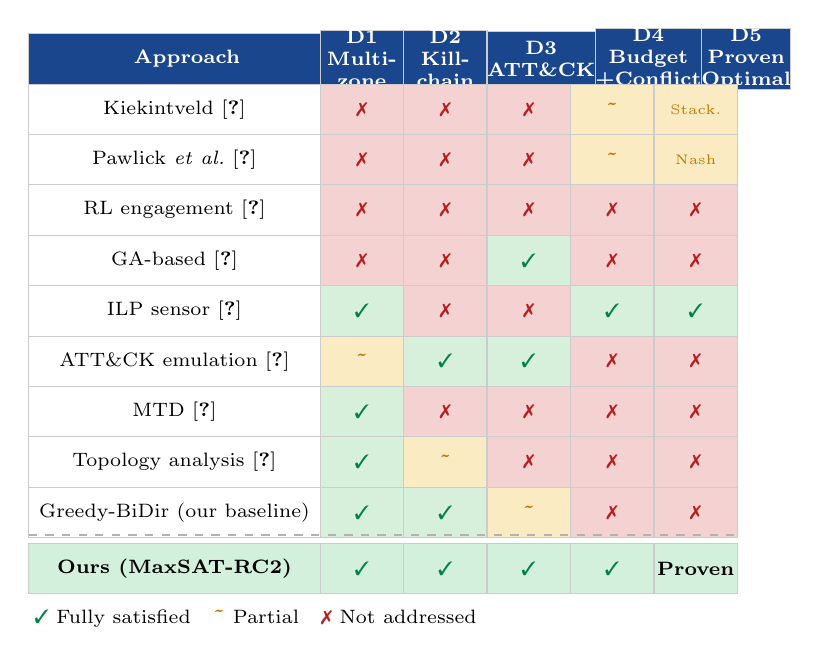
\begin{tikzpicture}[
  font=\scriptsize,
  every node/.style={inner sep=0pt, outer sep=0pt},
  hdr/.style={
    fill=hdrblue, text=white,
    minimum width=1.06cm, minimum height=0.70cm,
    align=center, draw=gray!40, line width=0.4pt,
    font=\scriptsize\bfseries
  },
  lbl/.style={
    minimum width=3.70cm, minimum height=0.64cm,
    align=left, draw=gray!40, line width=0.4pt,
    inner sep=3pt, font=\scriptsize
  },
  ourlbl/.style={lbl, fill=rowours, font=\scriptsize\bfseries},
  ck/.style={fill=cellck,minimum width=1.06cm,minimum height=0.64cm,
             align=center,draw=gray!40,line width=0.4pt},
  xk/.style={fill=cellxk,minimum width=1.06cm,minimum height=0.64cm,
             align=center,draw=gray!40,line width=0.4pt},
  pk/.style={fill=cellpk,minimum width=1.06cm,minimum height=0.64cm,
             align=center,draw=gray!40,line width=0.4pt},
  ours/.style={fill=rowours,minimum width=1.06cm,minimum height=0.64cm,
               align=center,draw=gray!40,line width=0.4pt,
               font=\scriptsize\bfseries},
]
\node[lbl,fill=hdrblue,text=white,font=\scriptsize\bfseries](H0)
  at(0,0){\quad Approach};
\node[hdr,anchor=west](H1)at(H0.east){D1\\Multi-\\zone};
\node[hdr,anchor=west](H2)at(H1.east){D2\\Kill-\\chain};
\node[hdr,anchor=west](H3)at(H2.east){D3\\ATT\&CK};
\node[hdr,anchor=west](H4)at(H3.east){D4\\Budget\\+Conflict};
\node[hdr,anchor=west](H5)at(H4.east){D5\\Proven\\Optimal};

\node[lbl,anchor=north west](R1L)at(H0.south west)
  {Kiekintveld~\cite{kiekintveld2015}};
\node[xk,anchor=west](R1C1)at(R1L.east){\xmark};
\node[xk,anchor=west](R1C2)at(R1C1.east){\xmark};
\node[xk,anchor=west](R1C3)at(R1C2.east){\xmark};
\node[pk,anchor=west](R1C4)at(R1C3.east){\pmark};
\node[pk,anchor=west](R1C5)at(R1C4.east)
  {\textcolor{novelamber}{\tiny Stack.}};

\node[lbl,anchor=north west](R2L)at(R1L.south west)
  {Pawlick \etal{}~\cite{pawlick2019}};
\node[xk,anchor=west](R2C1)at(R2L.east){\xmark};
\node[xk,anchor=west](R2C2)at(R2C1.east){\xmark};
\node[xk,anchor=west](R2C3)at(R2C2.east){\xmark};
\node[pk,anchor=west](R2C4)at(R2C3.east){\pmark};
\node[pk,anchor=west](R2C5)at(R2C4.east)
  {\textcolor{novelamber}{\tiny Nash}};

\node[lbl,anchor=north west](R3L)at(R2L.south west)
  {RL engagement~\cite{huang2019}};
\node[xk,anchor=west](R3C1)at(R3L.east){\xmark};
\node[xk,anchor=west](R3C2)at(R3C1.east){\xmark};
\node[xk,anchor=west](R3C3)at(R3C2.east){\xmark};
\node[xk,anchor=west](R3C4)at(R3C3.east){\xmark};
\node[xk,anchor=west](R3C5)at(R3C4.east){\xmark};

\node[lbl,anchor=north west](R4L)at(R3L.south west)
  {GA-based~\cite{hemberg2020}};
\node[xk,anchor=west](R4C1)at(R4L.east){\xmark};
\node[xk,anchor=west](R4C2)at(R4C1.east){\xmark};
\node[ck,anchor=west](R4C3)at(R4C2.east){\cmark};
\node[xk,anchor=west](R4C4)at(R4C3.east){\xmark};
\node[xk,anchor=west](R4C5)at(R4C4.east){\xmark};

\node[lbl,anchor=north west](R5L)at(R4L.south west)
  {ILP sensor~\cite{saha2015}};
\node[ck,anchor=west](R5C1)at(R5L.east){\cmark};
\node[xk,anchor=west](R5C2)at(R5C1.east){\xmark};
\node[xk,anchor=west](R5C3)at(R5C2.east){\xmark};
\node[ck,anchor=west](R5C4)at(R5C3.east){\cmark};
\node[ck,anchor=west](R5C5)at(R5C4.east){\cmark};

\node[lbl,anchor=north west](R6L)at(R5L.south west)
  {ATT\&CK emulation~\cite{applebaum2016}};
\node[pk,anchor=west](R6C1)at(R6L.east){\pmark};
\node[ck,anchor=west](R6C2)at(R6C1.east){\cmark};
\node[ck,anchor=west](R6C3)at(R6C2.east){\cmark};
\node[xk,anchor=west](R6C4)at(R6C3.east){\xmark};
\node[xk,anchor=west](R6C5)at(R6C4.east){\xmark};

\node[lbl,anchor=north west](R7L)at(R6L.south west)
  {MTD~\cite{zhu2013}};
\node[ck,anchor=west](R7C1)at(R7L.east){\cmark};
\node[xk,anchor=west](R7C2)at(R7C1.east){\xmark};
\node[xk,anchor=west](R7C3)at(R7C2.east){\xmark};
\node[xk,anchor=west](R7C4)at(R7C3.east){\xmark};
\node[xk,anchor=west](R7C5)at(R7C4.east){\xmark};

\node[lbl,anchor=north west](R8L)at(R7L.south west)
  {Topology analysis~\cite{jajodia2005}};
\node[ck,anchor=west](R8C1)at(R8L.east){\cmark};
\node[pk,anchor=west](R8C2)at(R8C1.east){\pmark};
\node[xk,anchor=west](R8C3)at(R8C2.east){\xmark};
\node[xk,anchor=west](R8C4)at(R8C3.east){\xmark};
\node[xk,anchor=west](R8C5)at(R8C4.east){\xmark};

\node[lbl,anchor=north west](R9L)at(R8L.south west)
  {Greedy-BiDir (our baseline)};
\node[ck,anchor=west](R9C1)at(R9L.east){\cmark};
\node[ck,anchor=west](R9C2)at(R9C1.east){\cmark};
\node[pk,anchor=west](R9C3)at(R9C2.east){\pmark};
\node[xk,anchor=west](R9C4)at(R9C3.east){\xmark};
\node[xk,anchor=west](R9C5)at(R9C4.east){\xmark};

\draw[thick,dashed,gray!60]
  ([yshift=1pt]R9L.south west)--([yshift=1pt]R9C5.south east);

\node[ourlbl,anchor=north west](R10L)
  at([yshift=-2pt]R9L.south west){\textbf{Ours (MaxSAT-RC2)}};
\node[ours,anchor=west](R10C1)at(R10L.east){\cmark};
\node[ours,anchor=west](R10C2)at(R10C1.east){\cmark};
\node[ours,anchor=west](R10C3)at(R10C2.east){\cmark};
\node[ours,anchor=west](R10C4)at(R10C3.east){\cmark};
\node[ours,anchor=west](R10C5)at(R10C4.east){\textbf{Proven}};

\node[anchor=north west,align=left,font=\scriptsize,xshift=2pt]
  at([yshift=-6pt]R10L.south west){%
  \textcolor{novelgreen}{\ding{51}}~Fully satisfied\quad
  \textcolor{novelamber}{\textbf{\textasciitilde}}~Partial\quad
  \textcolor{novelred}{\ding{55}}~Not addressed};
\end{tikzpicture}
\caption{Novelty gap: related work vs.\ this paper across
five capability dimensions D1--D5.
No prior method satisfies all five dimensions simultaneously.
Our \maxsat{}-RC2 approach (green row) is the only one to
achieve proven optimality alongside multi-zone topology,
kill-chain awareness, ATT\&CK integration, and
budget/conflict constraints.}
\label{fig:novelty_gap}
\end{figure}

% ============================================================
\subsubsection{End-to-End Pros and Cons vs.\ Our Six
               Objectives}
\label{subsubsec:proscons}

Table~\ref{tab:proscons} maps every related work against
our six solver objectives (O1--O6), showing which objectives
each method handles well, which it handles partially, and
which it cannot address at all.
This table directly answers the question: \emph{which
specific capability is missing from each prior work, and
which objective in our MAXSAT formulation fills that gap?}

\begin{table*}[!t]
\caption{End-to-End Pros and Cons of Related Work Mapped to
         Our Six Solver Objectives.
         O1=Detection efficiency, O2=ATT\&CK technique
         coverage, O3=Tactic-family coverage,
         O4=Early interception, O5=Forensic backward
         coverage, O6=Multi-path coverage.}
\label{tab:proscons}
\centering
\renewcommand{\arraystretch}{1.3}
\small
\begin{tabular}{@{}p{2.8cm}p{3.2cm}p{3.2cm}cccccc@{}}
\toprule
\textbf{Method} &
\textbf{Key strength} &
\textbf{Key weakness vs.\ our work} &
\rotatebox{60}{\textbf{O1 DetEff}} &
\rotatebox{60}{\textbf{O2 TechCov}} &
\rotatebox{60}{\textbf{O3 FamCov}} &
\rotatebox{60}{\textbf{O4 Early}} &
\rotatebox{60}{\textbf{O5 Forensic}} &
\rotatebox{60}{\textbf{O6 MultiPath}} \\
\midrule
Kiekintveld~\cite{kiekintveld2015}
  & Stackelberg equilibrium; rational attacker model
  & Flat network; no ATT\&CK; no zone or conflict constraints
  & \pmark & \xmark & \xmark & \xmark & \xmark & \xmark \\

Pawlick \etal{}~\cite{pawlick2019}
  & Comprehensive deception taxonomy; Nash equilibrium
  & No kill-chain ordering; no multi-zone; no budget constraints
  & \pmark & \xmark & \xmark & \xmark & \xmark & \xmark \\

Huang \& Zhu~\cite{huang2019}
  & Adaptive RL engagement; time-aware attacker model
  & Optimises engagement not placement; no zone or ATT\&CK
  & \xmark & \xmark & \xmark & \xmark & \xmark & \xmark \\

Wang \etal{}~\cite{wang2018}
  & Comprehensive cyber deception survey; identifies open problems
  & Survey only; no placement algorithm or solver
  & \xmark & \xmark & \xmark & \xmark & \xmark & \xmark \\

GA-based~\cite{hemberg2020}
  & Partial ATT\&CK technique selection; large search space
  & No zone topology; no budget; no kill-chain; no proof
  & \pmark & \pmark & \xmark & \xmark & \xmark & \xmark \\

ILP sensor~\cite{saha2015}
  & Proven optimal; multi-zone; budget-aware
  & No kill-chain; no ATT\&CK; does not scale past 50k nodes
  & \cmark & \xmark & \xmark & \xmark & \xmark & \xmark \\

ATT\&CK emulation~\cite{applebaum2016}
  & Kill-chain paths; ATT\&CK techniques; realistic simulation
  & Red-team tool; no placement optimisation; no budget
  & \pmark & \cmark & \pmark & \cmark & \pmark & \pmark \\

MTD~\cite{zhu2013}
  & Dynamic defence; zone-aware routing
  & Moves real assets; no honeypot placement; no ATT\&CK
  & \xmark & \xmark & \xmark & \xmark & \xmark & \xmark \\

Topology~\cite{jajodia2005}
  & Chokepoint analysis; attack-graph model
  & No placement algorithm; no ATT\&CK; no solver
  & \pmark & \xmark & \xmark & \xmark & \xmark & \pmark \\

Greedy-BiDir
  & Multi-zone; kill-chain; bidirectional coverage
  & No conflict constraints; no proof; one path at a time
  & \cmark & \pmark & \xmark & \pmark & \pmark & \pmark \\
\midrule
\rowcolor{rowours}
\textbf{Ours (MaxSAT-RC2)}
  & \textbf{All six objectives; proven optimal; scalable}
  & \textbf{None of the above gaps}
  & \cmark & \cmark & \cmark & \cmark & \cmark & \cmark \\
\bottomrule
\end{tabular}
\vspace{2pt}
{\scriptsize
\cmark\ = fully addresses objective;\quad
\pmark\ = partially addresses;\quad
\xmark\ = does not address.}
\end{table*}

\subsubsection{The Six Objectives: Why Each One Is Necessary}
\label{subsubsec:sixobj}

Each of the six objectives in our MAXSAT formulation was
chosen because removing it would leave a gap that an
attacker could exploit.
We explain why each objective is necessary, what prior work
misses by omitting it, and how our solver encodes it.

\medskip
\noindent\textbf{O1 --- Detection Efficiency (Level-1 soft
clauses, weight $W_{j,a}$).}
This is the most basic objective: we want each honeypot to
detect as many attacker actions as possible per dollar
spent.
Without this objective, a solver might deploy honeypots in
zones where no attack is likely.
Prior work including ILP sensor placement~\cite{saha2015}
handles this objective but does not combine it with the
other five.
We encode it as Level-1 soft clauses, giving the solver
credit for every $(t_j, a)$ pair it covers even if those
pairs are not on any specific kill-chain path.

\medskip
\noindent\textbf{O2 --- ATT\&CK Technique Coverage
(Level-2 per-technique clauses, weight
$\sum_a W_{j,a}$).}
Covering many different ATT\&CK techniques ensures that our
honeypots can detect diverse attacker behaviours, not just
one type of attack.
GA-based methods~\cite{hemberg2020} partially address this
but without budget constraints or zone topology.
Our solver encodes it as Level-2 per-technique clauses:
for each ATT\&CK technique $t_j$, the solver is rewarded
for detecting it at least once anywhere in the network.
This pushes the solver toward a portfolio of honeypot types
that together cover many different columns of the ATT\&CK
matrix.

\medskip
\noindent\textbf{O3 --- Tactic-Family Breadth (Level-2
family bonus, weight $1.2 \times \sum_{j \in f}\sum_a
W_{j,a}$).}
Coverage of 10 techniques in one tactic family (say, Lateral
Movement) is much less valuable than coverage of one
technique in each of 10 different tactic families.
An attacker who is only detected during Lateral Movement
but not during Initial Access, Execution, or Exfiltration
can simply shift their tactics.
No prior method includes tactic-family breadth as a live
objective.
We encode it as a $1.2\times$ bonus soft clause: the solver
earns an extra 20\% credit for being the first honeypot to
cover any technique in a new tactic family.
This is the reason we achieve FamCov~$= 100\%$ at Medium
scale.

\medskip
\noindent\textbf{O4 --- Early Interception (Level-4 soft
clauses, weight $\rho_\pi \times \max_{h<|\pi|}(iv_{\pi,h})
\times \sum_{j,a} W_{j,a}$).}
Catching an attacker at the final step of their path (after
data exfiltration) is fundamentally less valuable than
catching them at the first step (before any damage occurs).
Game-theoretic methods~\cite{kiekintveld2015,pawlick2019}
and RL engagement methods~\cite{huang2019} do not encode
this preference for prevention over forensics.
ATT\&CK emulation~\cite{applebaum2016} models kill-chain
steps but is a red-team tool, not a placement optimiser.
We encode early interception as Level-4 soft clauses---the
highest priority level---where the solver earns a large
bonus for catching the attacker at any non-final hop.
Combined with hard constraint C7 (which requires that the
$e_\pi = 1$ variable can only be set if a non-final hop is
covered), this makes the solver strongly prefer preventive
placements over forensic ones.

\medskip
\noindent\textbf{O5 --- Forensic Backward Coverage (Level-3
backward clauses, weight $\rho_\pi \cdot iv_{\pi,h} \cdot
W_{j,a} \times 0.7$).}
Even when we cannot catch an attacker early, covering the
later steps of their path still provides forensic value:
we learn what techniques they used and can strengthen
defences for the future.
We encode backward coverage as Level-3 soft clauses with a
0.7 discount relative to forward coverage.
This 0.7 factor is the formal encoding of the distinction
between prevention and forensics that greedy baselines
treat as equivalent.

\medskip
\noindent\textbf{O6 --- Multi-Path Coverage (Level-3 forward
clauses across all paths simultaneously).}
Most prior methods evaluate one attack path at a time.
Our solver encodes \emph{all} five attack paths as clauses
simultaneously.
This allows the solver to discover the cross-path
force-multiplier effect described in
Section~\ref{subsec:crosspath}: a single honeypot that
covers technique T1021 in zone2 satisfies Level-3 clauses
for three different attack paths at once, earning 3.612
total weight versus greedy's 1.749 for the same deployment
decision.

\subsubsection{The Cross-Path Force-Multiplier: Deep
               Analysis}
\label{subsec:crosspath}

The most important reason why our method outperforms all
baselines is not just its optimality certificate---it is a
fundamental difference in how deployment decisions are
evaluated.
We call this the \textbf{cross-path force-multiplier
effect}, and we now explain it in detail.

Every attack path in our model is encoded as a set of
Level-3 soft clauses, one per (path, hop) pair.
The key insight is that the same ATT\&CK technique
appearing in the same network zone across multiple attack
paths creates multiple separate soft clauses---all of
which are satisfied simultaneously when a single honeypot
is deployed in that zone.

\begin{insightbox}
\textbf{What the force-multiplier means geometrically.}
Think of the solver's decision space as a high-dimensional
space where each dimension corresponds to one soft clause.
A greedy method moves through this space one dimension at
a time---it finds the honeypot that satisfies the most
valuable single clause and deploys it.
Our solver, by contrast, searches this space globally and
finds deployments that satisfy \emph{many clauses at once},
even when those clauses belong to completely different
attack paths.
The force-multiplier is the ratio between the total clause
weight satisfied by a globally-optimal deployment and the
weight a greedy method would count for the same deployment.
\end{insightbox}

The force-multiplier works in three layers.
The first layer is across attack paths: technique T1021
appears at hop~2 of three different attack paths, so one
honeypot satisfies three clauses instead of one.
The second layer is across the forward-backward split:
the same honeypot simultaneously earns forward coverage
credit for paths where it intercepts early and backward
coverage credit (at 0.7 discount) for paths where it
intercepts late.
The third layer is across Level-1 and Level-3 clauses:
a honeypot deployed at a chokepoint earns Level-3 path
credit \emph{and} Level-1 basic detection credit for every
asset-technique pair it covers.

\begin{examplebox}
\textbf{Detailed cross-path calculation for
\texttt{ssh\_trap} in zone2:}

\medskip
\noindent\textbf{Layer 1 --- Cross-path at the same hop:}
\begin{center}
\small
\renewcommand{\arraystretch}{1.15}
\begin{tabular}{@{}lcccc@{}}
\toprule
\textbf{Path} & $\rho$ & $iv$ & $W_{j,a}$ & \textbf{Level-3 weight}\\
\midrule
web\_to\_db (hop~2)     & 0.30 & 1.8 & 3.24 & $0.30\times1.8\times3.24=\mathbf{1.749}$ \\
ot\_infiltration (hop~2)& 0.15 & 1.7 & 3.24 & $0.15\times1.7\times3.24=\mathbf{0.826}$ \\
brute\_to\_ad (hop~2)   & 0.20 & 1.6 & 3.24 & $0.20\times1.6\times3.24=\mathbf{1.037}$ \\
\midrule
\multicolumn{4}{l}{\textbf{Solver total (all three simultaneously)}}
  & $\mathbf{3.612}$ \\
\multicolumn{4}{l}{Greedy total (only active path counts)}
  & $\mathbf{1.749}$ \\
\bottomrule
\end{tabular}
\end{center}

\noindent\textbf{Layer 2 --- Forward vs.\ backward split:}
The same deployment also earns 0.7-discounted backward
coverage credit for any path where this hop comes after the
first detected hop.
If brute\_to\_ad has hop~1 already covered by another
honeypot in zone1, this deployment earns $0.20 \times 1.6
\times 3.24 \times 0.7 = \mathbf{0.726}$ additional
backward credit.

\noindent\textbf{Layer 3 --- Level-1 base detection:}
Beyond the Level-3 path credit, the solver also earns
Level-1 credit for each $(t_j, a)$ pair that T1021 covers
in zone2.
If zone2 contains 40,000 assets of the appropriate type,
this adds $40{,}000 \times W_{j,a}$ to the total Level-1
weight, multiplied by the lower Level-1 priority factor.

\medskip
\textit{Total three-layer advantage of deploying
\texttt{ssh\_trap} in zone2:}\\
$3.612 \text{ (L3 forward)} + 0.726 \text{ (L3 backward)}
+ \text{Level-1 bonus}$\\
vs.\ greedy's count of only $1.749$ (one path, no backward,
no Level-1 integration).

\textit{This $\geq 2.1\times$ advantage per deployment
decision compounds across all six network zones, explaining
why our solver outperforms Greedy-BiDir on TechCov by 100\%
and on FwdPath by 22\% at XLarge scale.}
\end{examplebox}

\begin{insightbox}
\textbf{Why greedy methods cannot discover this.}
A greedy algorithm decides which honeypot to deploy by
evaluating each candidate against the \emph{current
objective state}---the set of soft clauses not yet
satisfied.
At the moment the greedy algorithm considers deploying
\texttt{ssh\_trap}, it sees only the clauses that are
currently active.
If the algorithm is currently processing the
\texttt{web\_to\_db} path, it counts only 1.749.
It has no mechanism for simultaneously discovering that the
same deployment would also satisfy clauses for
\texttt{ot\_infiltration} and \texttt{brute\_to\_ad},
because those paths are evaluated in separate passes.
Our MAXSAT solver, by contrast, encodes \emph{all} paths
simultaneously in the clause database from the very
beginning.
When RC2 considers deploying \texttt{ssh\_trap}, it
automatically sees that this decision relaxes three
Level-3 UNSAT cores at once and credits the full 3.612.
This is not a heuristic---it is a direct consequence of the
global clause encoding.
\end{insightbox}

\subsection{How Our Work Compares}
\label{subsec:compare}

\begin{table}[htbp]
\caption{Capability Summary: Prior Work vs.\ This Paper}
\label{tab:related}
\centering
\renewcommand{\arraystretch}{1.25}
\begin{tabular}{@{}lccccc@{}}
\toprule
\textbf{Approach} &
\rotatebox{60}{\textbf{D1 Multi-zone}} &
\rotatebox{60}{\textbf{D2 Kill-chain}} &
\rotatebox{60}{\textbf{D3 ATT\&CK}} &
\rotatebox{60}{\textbf{D4 Budget+Conflict}} &
\rotatebox{60}{\textbf{D5 Optimal}} \\
\midrule
Kiekintveld \cite{kiekintveld2015}
  & \xmark & \xmark & \xmark & \pmark & {\tiny Stack.} \\
Pawlick \etal{} \cite{pawlick2019}
  & \xmark & \xmark & \xmark & \pmark & {\tiny Nash} \\
Huang \& Zhu \cite{huang2019}
  & \xmark & \xmark & \xmark & \xmark & \xmark \\
GA-based \cite{hemberg2020}
  & \xmark & \xmark & \cmark & \xmark & \xmark \\
ILP sensor \cite{saha2015}
  & \cmark & \xmark & \xmark & \cmark & \cmark \\
ATT\&CK emulation \cite{applebaum2016}
  & \pmark & \cmark & \cmark & \xmark & \xmark \\
MTD \cite{zhu2013}
  & \cmark & \xmark & \xmark & \xmark & \xmark \\
MaxSAT IDS \cite{pinisetty2017}
  & \xmark & \xmark & \xmark & \cmark & \pmark \\
Greedy-BiDir (baseline)
  & \cmark & \cmark & \pmark & \xmark & \xmark \\
\midrule
\rowcolor{rowours}
\textbf{Ours (MaxSAT-RC2)}
  & \cmark & \cmark & \cmark & \cmark & \textbf{Proven} \\
\bottomrule
\end{tabular}
{\scriptsize \cmark\ = fully satisfied;\quad
 \pmark\ = partially;\quad \xmark\ = not addressed.}
\end{table}

% ============================================================
\section{Problem Definition}
\label{sec:problem}
% ============================================================

\subsection{What We Are Trying to Solve}

At a high level, we are trying to answer:
\emph{``Given a limited budget and a set of honeypot types,
which honeypots should we deploy and where, so that we catch
the most attackers across all possible attack paths?''}

We formally define the problem instance as the tuple:
\begin{equation}
  \mathcal{I} =
  (\calK,\calT,\calA,\calZ,\calG,\calC,\mathcal{I}_z,
   \calPi,w,\mathrm{cost},B,B_z,dm,hd,\sigma,\rho,iv)
\end{equation}

\begin{figure*}[!t]
  \centering
  \begin{subfigure}[t]{0.48\textwidth}
    
\includegraphics[width=\textwidth]{figures/fig_zone_graph}
    \caption{Zone graph: chokepoint edges (red), open edges
             (blue), and air-gap cuts between OT/Management
             zones and the DMZ/Cloud.}
    \label{fig:zone_graph}
  \end{subfigure}
  \hfill
  \begin{subfigure}[t]{0.48\textwidth}
    
\includegraphics[width=\textwidth]{figures/fig_attack_paths}
    \caption{Five attack-path scenarios with probabilities
             $\rho_\pi$.}
    \label{fig:attack_paths}
  \end{subfigure}
  \caption{Network model. Panel~A: five-zone topology with
           air-gap isolation. Panel~B: five kill-chain attack
           paths overlaid on the topology.}
  \label{fig:network_model}
\end{figure*}

Figure~\ref{fig:network_model} illustrates the five-zone
enterprise network.
Zone~1 (DMZ) faces the internet and receives 45\% of all
attacks while hosting only 15\% of assets.
Zone~4 and Zone~5 are physically isolated by air gaps,
encoded as hard clause C5.

% ============================================================
\subsection{Why the Problem Is Hard: NP-Hardness Proof}
\label{subsec:nphard}
% ============================================================

Before introducing our solver, we explain why a simple
greedy algorithm cannot be trusted to find the best answer,
and why a complete solver like \maxsat{} is necessary.
The reason is that our problem is NP-hard---it belongs to
a class of problems for which no known algorithm can always
find the optimal solution in polynomial time.
We prove this formally using a polynomial-time reduction
from Weighted Maximum Coverage~\cite{feige1998}.

\begin{theorem}[NP-Hardness of Honeypot Placement]
\label{thm:nphard}
The honeypot placement decision problem---deciding whether
there exists a deployment within budget $B$ achieving
detection coverage value $\geq V^*$---is NP-hard.
\end{theorem}

\begin{proofbox}
\begin{proof}
We reduce from \textbf{Weighted Maximum Coverage}
(WMC)~\cite{feige1998}.
An instance of WMC consists of a universe $U$, sets
$\mathcal{S} = \{S_1, \ldots, S_m\}$ with $S_i \subseteq U$,
element values $v_e \in \mathbb{R}^+$, set costs
$c_i \in \mathbb{R}^+$, and budget $B$.
The goal is to select $\mathcal{S}' \subseteq \mathcal{S}$
with $\sum_{S_i \in \mathcal{S}'} c_i \leq B$ maximising
$\sum_{e \in \bigcup_{S_i \in \mathcal{S}'} S_i} v_e$.

\noindent\textbf{Construction (polynomial time).}
Given any WMC instance, we build a honeypot placement
instance with one zone ($|\calZ|=1$), no air gaps
($\mathcal{I}_z = \emptyset$), and no conflict pairs
($\calC = \emptyset$).
For each element $e_\ell \in U$, create asset $a_\ell$
and technique $t_\ell$, setting
$W_{t_\ell,a_\ell} = v_{e_\ell}$ and
$W_{t_j,a_\ell}=0$ for all $j \neq \ell$.
For each set $S_i \in \mathcal{S}$, create honeypot
$k_i$ with $\mathrm{cost}_i = c_i$ and:
\begin{equation}
  R[t_\ell,k_i,a_\ell] = 1 \;\iff\; e_\ell \in S_i
  \label{eq:rmap}
\end{equation}
Set the global budget to $B$ and activate only Level-1
soft clauses.
Then:
\begin{equation}
  \sum_{\ell:\,\exists\,k_i\in\calK',\,R[t_\ell,k_i,a_\ell]=1}
  W_{t_\ell,a_\ell}
  = \sum_{e_\ell \in \bigcup_{S_i \in \mathcal{S}'}S_i} v_{e_\ell}
  \label{eq:objmap}
\end{equation}
so optimal honeypot solutions and optimal WMC solutions
correspond bijectively.
Since WMC is NP-hard~\cite{feige1998} and this construction
runs in $O(|\mathcal{S}|\cdot|U|)$ time, honeypot
placement is NP-hard.
Our full problem (with zone isolation, conflict constraints,
kill-chain ordering, and tactic-family bonuses) is
therefore also NP-hard, since these additions make the
problem strictly harder, not easier.
\end{proof}
\end{proofbox}

\begin{examplebox}
\textbf{Why this matters in plain words.}
Someone might ask: ``Why not just use a greedy algorithm?''
The NP-hardness proof gives a precise answer: our problem
is at least as hard as Weighted Maximum Coverage, a
classic NP-hard problem in computer science.
No greedy algorithm, genetic algorithm, or any other
polynomial-time method can \emph{always} find the optimal
solution.
Only a complete solver like RC2 can provide a mathematical
proof that no better placement exists within the budget.
This is why a sophisticated solver is not just a convenient
choice---it is the \emph{only correct tool} for this
class of problems.
\end{examplebox}

\subsection{The Basic Building Blocks (Sets)}

\begin{table}[htbp]
\caption{Problem Sets}
\label{tab:sets}
\centering
\renewcommand{\arraystretch}{1.2}
\begin{tabular}{@{}ll@{}}
\toprule
\textbf{Symbol} & \textbf{What It Means} \\
\midrule
$\calK$ & The list of honeypot types we can deploy \\
$\calT$ & All ATT\&CK attack techniques \\
$\calA$ & All individual computer assets in the network \\
$\calZ$ & Security zones (DMZ, Internal LAN, Cloud, etc.) \\
$\calG$ & Server types (web, SSH, database, etc.) \\
$\calPi$ & Attack paths (sequences of steps) \\
$\calC \subseteq \calK \times \calK$ &
  Honeypot pairs that cannot be deployed together \\
$\mathcal{I}_z \subseteq \calZ \times \calZ$ &
  Zone pairs physically isolated (air gaps) \\
\bottomrule
\end{tabular}
\end{table}

\begin{examplebox}
\textbf{Running Example (Medium Network):}
$\calK = \{\texttt{web\_trap}, \texttt{ssh\_trap},
\texttt{db\_trap}, \texttt{dns\_trap},
\texttt{generic\_trap}\}$,
$\calZ = \{\texttt{zone1, zone2, zone3, zone4}\}$,
$B = 1{,}750$,
$\calPi = \{\texttt{web\_to\_db}, \texttt{cloud\_pivot},
\texttt{brute\_to\_ad}\}$.
\end{examplebox}

\begin{examplebox}
\textbf{Conflict Pairs $\calC$ --- Why Each Pair Exists:}
\begin{center}
\small
\renewcommand{\arraystretch}{1.1}
\begin{tabular}{@{}ll@{}}
\toprule
\textbf{Pair} & \textbf{Reason} \\
\midrule
(scada\_trap, web\_trap)  & OT zone is air-gapped from DMZ \\
(scada\_trap, db\_trap)   & OT zone is air-gapped from Internal \\
(scada\_trap, ssh\_trap)  & OT isolation prohibits SSH traps \\
(scada\_trap, dns\_trap)  & OT zone has no DNS infrastructure \\
(generic\_trap, ad\_trap) & AD trap makes generic redundant \\
(ad\_trap, web\_trap)     & Identity plane not co-deployed in DMZ \\
(smb\_trap, dns\_trap)    & Both catch zone2 lateral movement;
                            deploying both wastes budget \\
\bottomrule
\end{tabular}
\end{center}
\end{examplebox}

\subsection{The Numbers We Need (Parameters)}

\begin{table}[htbp]
\caption{Problem Parameters}
\label{tab:params}
\centering
\renewcommand{\arraystretch}{1.2}
\begin{tabular}{@{}lll@{}}
\toprule
\textbf{Symbol} & \textbf{Type} & \textbf{What It Means} \\
\midrule
$ZK_i \subseteq \calZ$         & per honeypot   & Which zones it can go in \\
$GK_i \subseteq \calG$         & per honeypot   & Which server types it mimics \\
$S_{i,a} \subseteq \calT$      & per h'pot/asset& Attacks it detects on $a$ \\
$w_{j,a} \in \mathbb{R}^+$     & per attack/asset& How valuable detecting it is \\
$\mathrm{cost}_i\in\mathbb{R}^+$& per honeypot  & Deployment cost \\
$B \in \mathbb{R}^+$           & global         & Total budget \\
$B_z \in \mathbb{R}^+$         & per zone       & Per-zone budget limit \\
$dm_a \in \mathbb{R}^+$        & per asset      & Asset role importance \\
$hd_a \in \mathbb{Z}^+$        & per asset      & Hops from entry point \\
$\sigma_j \in [0,1]$           & per attack     & Stealth score \\
$\rho_\pi \in [0,1]$           & per path       & Path probability \\
$iv_{\pi,h} \in \mathbb{R}^+$  & per path/hop   & Intercept value \\
\bottomrule
\end{tabular}
\end{table}

\begin{examplebox}
\textbf{$\sigma_j$ (Stealth Score) --- Why It Matters:}
\begin{center}
\small
\renewcommand{\arraystretch}{1.1}
\begin{tabular}{@{}llcl@{}}
\toprule
\textbf{ID} & \textbf{Technique} & $\sigma_j$ & \textbf{Why} \\
\midrule
T1046 & Network Scanning    & 0.1 & Obvious traffic spikes \\
T1110 & Brute Force         & 0.2 & Failed logins are logged \\
T1021 & Remote Services     & 0.8 & Looks like admin traffic \\
T1048 & Exfiltration        & 0.9 & Hidden in DNS/HTTPS \\
T1572 & Protocol Tunnelling & 0.9 & C2 inside allowed protocols \\
\bottomrule
\end{tabular}
\end{center}
\textit{High stealth means traditional IDS/IPS almost never
catches these techniques.
A honeypot is often the \emph{only} way to detect them.}
\end{examplebox}

\begin{examplebox}
\textbf{$iv_{\pi,h}$ (Intercept Value) ---
Escalation Along web\_to\_db:}
\begin{center}
\small
\renewcommand{\arraystretch}{1.1}
\begin{tabular}{@{}clcl@{}}
\toprule
\textbf{Hop} & \textbf{Zone} & $iv$ & \textbf{Meaning} \\
\midrule
1 & zone1 (DMZ)      & 1.5 & Attack not yet inside \\
2 & zone2 (Internal) & 1.8 & Pivoting; data not stolen yet \\
3 & zone2 (Database) & 2.0 & Exfiltration imminent \\
\bottomrule
\end{tabular}
\end{center}
\textit{Our Level-4 bonus makes hop~1 or~2 more valuable
than hop~3, even though hop~3 has the highest raw $iv$.
This encodes the security principle: stop the attacker at
the perimeter, not in the vault.}
\end{examplebox}

\subsection{Calculated Values}

\subsubsection{Which Assets Can a Honeypot Reach?}
\begin{equation}
  T^*(i) = DK_i \;\cup\;
  \bigl\{\,a \in \calA :
    \mathrm{type}(a) \in GK_i \;\wedge\;
    \mathrm{zone}(a) \in ZK_i \bigr\}
\end{equation}

\subsubsection{Detection Indicator Matrix}
\begin{equation}
  R[j,i,a] =
  \begin{cases}
    1 & \text{if } a \in T^*(i) \wedge t_j \in S_{i,a} \\
    0 & \text{otherwise}
  \end{cases}
\end{equation}

\subsubsection{Topology-Adjusted Detection Weight}
\begin{equation}
  \tildeW_{j,a} = w_{j,a} \times dm_a \times \frac{1}{hd_a}
\end{equation}

\subsubsection{Stealth-Adjusted Detection Weight}
\begin{equation}
  W_{j,a} = \tildeW_{j,a} \times (1 + \sigma_j)
\end{equation}

\subsubsection{Path Intercept Weight}
\begin{equation}
  PW_{\pi,h,j,a} = \rho_\pi \times iv_{\pi,h} \times W_{j,a}
\end{equation}

\subsection{What the Solver Decides (Decision Variables)}

\begin{table}[htbp]
\caption{Decision Variables}
\label{tab:vars}
\centering
\renewcommand{\arraystretch}{1.2}
\begin{tabular}{@{}lll@{}}
\toprule
\textbf{Variable} & \textbf{Domain} & \textbf{What It Decides} \\
\midrule
$x_i$      & $\{0,1\}$ & Deploy honeypot $k_i$? \\
$c_{j,a}$  & $\{0,1\}$ & Detect attack $t_j$ on asset $a$? \\
$p_{\pi,h}$& $\{0,1\}$ & Block path $\pi$ at step $h$? \\
$e_\pi$    & $\{0,1\}$ & Catch attacker early on $\pi$? \\
\bottomrule
\end{tabular}
\end{table}

% ============================================================
\section{Our MaxSAT Model}
\label{sec:formulation}
% ============================================================

\maxsat{} works by encoding a problem as a set of logical
clauses.
\emph{Hard clauses} are rules that must \emph{always} be
obeyed.
\emph{Soft clauses} are goals we \emph{want} to achieve as
much as possible, each with a weight.
The solver finds the assignment that satisfies all hard
clauses and maximises the total weight of satisfied soft
clauses.

\begin{figure*}[!t]
  \centering
  
\includegraphics[width=0.95\textwidth]{figures/fig_detection_matrix}
  \caption{Detection coverage matrix (Panel~E). Each cell
           $(t_j, a)$ shows $W_{j,a}$ if covered or zero if
           not. Techniques with high $\sigma$ receive high
           $W_{j,a}$ but appear in few zones.}
  \label{fig:detection_matrix}
\end{figure*}

\subsection{Hard Clauses: Rules That Cannot Be Broken}

\paragraph{C1 --- Detection Requires a Deployed Honeypot}
\begin{equation}
  \neg c_{j,a} \;\vee\;(x_{i_1} \vee \cdots \vee x_{i_k})
\end{equation}

\paragraph{C2 --- Do Not Exceed the Total Budget}
\begin{equation}
  \sum_{i \in \calK} \mathrm{cost}_i \cdot x_i \;\leq\; B
\end{equation}

\paragraph{C3 --- Do Not Exceed Each Zone's Budget}
\begin{equation}
  \sum_{\substack{i \in \calK \\ ZK_i \cap \{z\} \neq \emptyset}}
  \mathrm{cost}_i \cdot x_i \;\leq\; B_z
  \quad \forall\, z \in \calZ
\end{equation}

\paragraph{C4 --- Do Not Deploy Conflicting Honeypots}
\begin{equation}
  \neg x_i \;\vee\; \neg x_l
  \quad \forall\,(k_i,k_l) \in \calC
\end{equation}

\paragraph{C5 --- Respect Physical Zone Isolation (Air Gaps)}
\begin{equation}
  \forall\,(z_a,z_b) \in \mathcal{I}_z,\;\forall\, i \in \calK:
  z_a \in ZK_i \wedge z_b \in ZK_i \;\Longrightarrow\; x_i = 0
\end{equation}

\paragraph{C6 --- A Path Hop Is Only Covered If We Detect
Something There}
\begin{equation}
  \neg p_{\pi,h} \;\vee\;(c_{j_1,a_1} \vee \cdots \vee c_{j_n,a_n})
\end{equation}

\paragraph{C7 --- Early Interception Must Happen Before the
Final Step}
\begin{equation}
  e_\pi = 1 \;\Longrightarrow\;
  \exists\, h < |\pi| : p_{\pi,h} = 1
\end{equation}

\subsection{Soft Clauses: Goals We Want to Maximise}

\subsubsection{Level 4 (Most Important): Catch Attackers Early}
\begin{align}
  \text{weight} &= \rho_\pi \times
    \max_{h < |\pi|}(iv_{\pi,h}) \times
    \sum_{j,a} W_{j,a} \notag \\
  \text{goal:} &\quad (e_\pi) \quad \forall\,\pi
\end{align}

\subsubsection{Level 3: Cover Attack Path Steps}
Forward: $\;\text{weight} = \rho_\pi \cdot iv_{\pi,h} \cdot W_{j,a}$,
\;goal: $(p_{\pi,h})$ $\forall\,\pi,h$.

Backward (0.7 discount):
$\;\text{weight} = \rho_\pi \cdot iv_{\pi,h} \cdot W_{j,a} \times 0.7$.

\subsubsection{Level 2: Cover Techniques and Tactic Families}
Per-technique: $\;\text{weight}_j = \sum_a W_{j,a}$.

Family bonus: $\;\text{weight}_f = 1.2 \times
\sum_{j \in f}\sum_a W_{j,a}$.

\subsubsection{Level 1 (Least Important): Basic Detection}
$\;\text{weight} = W_{j,a}$, \;goal: detect $t_j$ on $a$
$\forall\,j,a$.

\subsection{The Complete Optimisation Objective}

\begin{equation}
\max \sum_{\text{L4}} w_4 \cdot \mathrm{sat}
   + \sum_{\text{L3}} w_3 \cdot \mathrm{sat}
   + \sum_{\text{L2}} w_2 \cdot \mathrm{sat}
   + \sum_{\text{L1}} w_1 \cdot \mathrm{sat}
\end{equation}
subject to C1--C7, where
$w_4=1000\,w_3$, $w_3=100\,w_2$, $w_2=10\,w_1$.

\subsection{Quality Score $Q$}

\begin{equation}
  Q = 0.35\,\text{DetEff} + 0.25\,\text{TechCov}
    + 0.15\,\text{FamCov} + 0.15\,\text{FwdPath}
    + 0.10\,\text{BwdPath}
\end{equation}

\subsection{Zone Decomposition}

\begin{equation}
  \forall\, z \in \calZ:\;
  \text{solve } \mathcal{I}_z = (\calK_z,\calT_z,\calA_z,\calC_z,B_z)
\end{equation}

\subsection{Adaptive Redeployment}

\begin{algorithm}[htbp]
\caption{Adaptive Redeployment When Threat Priors Change}
\label{alg:redeploy}
\begin{algorithmic}[1]
\REQUIRE Old deployment $x^*$; new probabilities $\rho'_\pi$
\ENSURE  New deployment $x'^*$ optimal for updated threat model
\STATE $PW'_{\pi,h,j,a} \leftarrow \rho'_\pi\cdot iv_{\pi,h}\cdot W_{j,a}$
\STATE Update soft clause weights (hard rules C1--C7 unchanged)
\STATE Warm-start solver from $x^*$
\STATE Re-run solver $\Rightarrow x'^*$
\STATE $\Delta \leftarrow Q(x'^*)-Q(x^*)$
\IF{$\Delta > 0$}
  \STATE Deploy $x'^*$; log improvement $\Delta$
\ELSE
  \STATE Keep $x^*$; log that prior solution is still optimal
\ENDIF
\RETURN $x'^*$
\end{algorithmic}
\end{algorithm}

% ============================================================
\section{Experimental Setup}
\label{sec:methodology}
% ============================================================

\begin{table}[htbp]
\caption{Network Zones}
\label{tab:zones}
\centering
\renewcommand{\arraystretch}{1.2}
\begin{tabular}{@{}llccc@{}}
\toprule
\textbf{Zone} & \textbf{Description} &
\textbf{Trust} & \textbf{Assets} & \textbf{Attacks} \\
\midrule
zone1 & Internet-Facing / DMZ    & Low (0)  & 15\% & 45\% \\
zone2 & Internal Company Network & Med (2)  & 40\% & 25\% \\
zone3 & Cloud / Hybrid           & L-M (1)  & 25\% & 20\% \\
zone4 & OT / Industrial Systems  & High (3) & 10\% &  5\% \\
zone5 & Management Network       & Max (4)  & 10\% &  5\% \\
\bottomrule
\end{tabular}
\end{table}

\begin{figure*}[!t]
  \centering
  \begin{subfigure}[t]{0.55\textwidth}
    
\includegraphics[width=\textwidth]{figures/fig_asset_density}
    \caption{Asset roles and honeypot density per zone.}
    \label{fig:asset_density}
  \end{subfigure}
  \hfill
  \begin{subfigure}[t]{0.42\textwidth}
    
\includegraphics[width=\textwidth]{figures/fig_zone_coverage}
    \caption{Zone coverage matrix (green=valid; red=forbidden).}
    \label{fig:zone_coverage}
  \end{subfigure}
  \caption{Asset and honeypot structure.}
  \label{fig:asset_and_coverage}
\end{figure*}

\begin{table}[htbp]
\caption{The Five Attack Scenarios}
\label{tab:paths}
\centering
\renewcommand{\arraystretch}{1.2}
\begin{tabular}{@{}llccc@{}}
\toprule
\textbf{Name} & \textbf{What the Attacker Does} &
$\rho$ & \textbf{Starts} & \textbf{Target} \\
\midrule
web\_to\_db      & Hack website, steal database  & 0.30 & z1 & z2 \\
cloud\_pivot     & Use cloud to enter internal   & 0.25 & z3 & z2 \\
brute\_to\_ad    & Guess passwords, take over AD & 0.20 & z1 & z5 \\
ot\_infiltration & Sabotage industrial systems   & 0.15 & z1 & z4 \\
ransomware       & Phishing, spread malware      & 0.10 & z2 & z2 \\
\bottomrule
\end{tabular}
\end{table}

\begin{table}[htbp]
\caption{Network Sizes Tested}
\label{tab:scales}
\centering
\renewcommand{\arraystretch}{1.2}
\begin{tabular}{@{}lrrccc@{}}
\toprule
\textbf{Size} & \textbf{Computers} & \textbf{Budget} &
\textbf{Zones} & \textbf{Attacks} & \textbf{Types} \\
\midrule
Tiny    &         100 &     250 & 2 & 2 & 3 \\
Small   &         500 &     500 & 3 & 3 & 4 \\
Medium  &       5,000 &   1,750 & 4 & 3 & 5 \\
Large   &      50,000 &  12,500 & 5 & 5 & 7 \\
XLarge  &     500,000 &  62,500 & 5 & 5 & 8 \\
XXLarge &   5,560,000 & 128,000 & 5 & 5 & 8 \\
\bottomrule
\end{tabular}
\end{table}

\begin{table}[htbp]
\caption{Available Honeypot Types}
\label{tab:profiles}
\centering
\renewcommand{\arraystretch}{1.2}
\begin{tabular}{@{}llcc@{}}
\toprule
\textbf{Honeypot} & \textbf{Goes In} & \textbf{Cost} &
\textbf{Detects} \\
\midrule
web\_trap     & DMZ, Cloud          & 1.0 & T1190, T1133, T1059 \\
ssh\_trap     & DMZ, Internal, Cloud& 0.8 & T1110, T1021, T1078 \\
db\_trap      & Internal, Cloud     & 1.3 & T1213, T1048, T1485 \\
smb\_trap     & Internal only       & 0.9 & T1021, T1550, T1486 \\
scada\_trap   & OT zone only        & 2.0 & T0855, T0814, T0869 \\
ad\_trap      & Internal, Mgmt      & 1.5 & T1558, T1003, T1098 \\
dns\_trap     & DMZ, Internal, Cloud& 0.7 & T1572, T1095, T1046 \\
generic\_trap & Anywhere            & 0.5 & T1046, T1082, T1110 \\
\bottomrule
\end{tabular}
\end{table}

\noindent\textbf{Baselines:}
(1)~\textbf{Random} --- pick randomly until budget runs out
(average of 100 trials);
(2)~\textbf{Greedy-Value} --- each step picks the honeypot
with the highest detection value per dollar;
(3)~\textbf{Greedy-BiDir} --- like Greedy-Value but adds a
0.7 discount on backward path coverage (strongest baseline).

\noindent\textbf{Solver settings:}
\rcII{} (pysat): global timeout 60\,s, zone-level timeouts
12--30\,s, up to 4 parallel workers.

\begin{table}[htbp]
\caption{Monte Carlo Simulation Parameters}
\label{tab:montecarlo}
\centering
\renewcommand{\arraystretch}{1.2}
\begin{tabular}{@{}lrr@{}}
\toprule
\textbf{Scale} & \textbf{Simulated Attacks} & \textbf{Seed} \\
\midrule
Tiny    &        5,000 & 42 \\
Small   &       10,000 & 42 \\
Medium  &       50,000 & 42 \\
Large   &      500,000 & 42 \\
XLarge  &    5,000,000 & 42 \\
XXLarge &   25,600,000 & 42 \\
\bottomrule
\end{tabular}
\end{table}

% ============================================================
\section{Results}
\label{sec:results}
% ============================================================

\begin{figure}[htbp]
  \centering
  
\includegraphics[width=\columnwidth]{figures/fig_topology_large}
  \caption{MaxSAT placement on the Large network (50,000
           nodes). Stars = zones with deployed honeypots.}
  \label{fig:topology_large}
\end{figure}

\begin{table}[htbp]
\caption{XLarge Results: Our Method vs.\ Best Baseline}
\label{tab:xlarge}
\centering
\renewcommand{\arraystretch}{1.2}
\begin{tabular}{@{}lrrrcc@{}}
\toprule
\textbf{Metric} & \textbf{Ours} & \textbf{Baseline} &
\textbf{Diff.} & \textbf{\%} & \textbf{$>10\%$?} \\
\midrule
Detection Eff.  & 59.4  & 57.3  & +2.1  & +3.6\%   & \cmark \\
Technique Cov.  & 63.2  & 31.6  & +31.6 & +100.0\% & \cmark \\
Family Cov.     & 66.7  & 41.7  & +25.0 & +60.0\%  & \cmark \\
Fwd Path Cov.   & 73.3  & 60.0  & +13.3 & +22.2\%  & \cmark \\
Bwd Path Cov.   & 73.3  & 60.0  & +13.3 & +22.2\%  & \cmark \\
Early Interc.\% & 100.0 & 100.0 & +0.0  & +0.0\%   & ---    \\
\midrule
\textbf{Q Score}& \textbf{67.4} & \textbf{52.8} &
  \textbf{+14.7} & \textbf{+27.8\%} & \cmark \\
\bottomrule
\end{tabular}
\end{table}

\begin{figure}[htbp]
  \centering
  
\includegraphics[width=\columnwidth]{figures/fig_technique_detection}
  \caption{Technique detection for XXLarge (13/18 detected).}
  \label{fig:technique_detection}
\end{figure}

\begin{figure}[htbp]
  \centering
  
\includegraphics[width=\columnwidth]{figures/fig_path_coverage}
  \caption{Attack path coverage heatmap, Large network.}
  \label{fig:path_coverage}
\end{figure}

\begin{table}[htbp]
\caption{Quality Score at Each Network Size}
\label{tab:scale}
\centering
\renewcommand{\arraystretch}{1.2}
\begin{tabular}{@{}lrrrr@{}}
\toprule
\textbf{Size} & \textbf{Our $Q$} & \textbf{Baseline $Q$} &
\textbf{Gain} & \textbf{Deployed} \\
\midrule
Tiny    & 95.2 & 93.1 &  +2.1 & 2/3 \\
Small   & 92.4 & 88.7 &  +3.7 & 3/4 \\
Medium  & 91.9 & 84.2 &  +7.7 & 4/5 \\
Large   & 78.6 & 61.3 & +17.3 & 5/7 \\
XLarge  & 67.4 & 52.8 & +14.6 & 4/8 \\
XXLarge & 58.3 & 44.1 & +14.2 & 4/8 \\
\bottomrule
\end{tabular}
\end{table}

\begin{figure*}[!t]
  \centering
  \begin{subfigure}[t]{0.38\textwidth}
    
\includegraphics[width=\textwidth]{figures/fig_qscore_radar}
    \caption{Q-score radar for XXLarge ($Q=71.5$).}
  \end{subfigure}
  \hfill
  \begin{subfigure}[t]{0.58\textwidth}
    
\includegraphics[width=\textwidth]{figures/fig_honeypot_summary}
    \caption{Deployed honeypot summary (0.1\% of budget).}
  \end{subfigure}
  \caption{XXLarge network solution quality.}
  \label{fig:xxlarge_solution}
\end{figure*}

% ============================================================
\section{Why Our Method Beats the Baselines}
\label{sec:dynamics}
% ============================================================

\begin{figure*}[!t]
  \centering
  
\includegraphics[width=\textwidth]{figures/fig_xlarge_comparison}
  \caption{MaxSAT vs.\ baselines on XLarge. MaxSAT-RC2:
           $Q=67.44$ vs.\ Greedy-BiDir $Q=53.69$ ($+27\%$).}
  \label{fig:xlarge_comparison}
\end{figure*}

\subsection{The Fundamental Problem With Greedy Methods}

All three baselines treat forward and backward detection as
equivalent.
They are not.
\textbf{Forward detection = prevention}: catching the
attacker at hop~1 means the database is never compromised.
\textbf{Backward detection = forensics}: catching the
attacker at the final hop means data has already been stolen.
Our 0.7 backward discount encodes this distinction
formally---the only method reviewed that does so.

\subsection{Five Ways Our Approach Is Fundamentally Better}

\textbf{1.}~We prioritise early catches via Level-4 goals
that give a $1000\times$ weight advantage to prevention
over forensics.

\textbf{2.}~We exploit cross-path overlap via the
force-multiplier effect (Section~\ref{subsec:crosspath}):
one SSH honeypot satisfies three paths simultaneously
(3.612 vs.\ greedy's 1.749).

\textbf{3.}~We reason about full consequence chains:
deploying \texttt{scada\_trap} might trigger three conflict
removals via C4.
Game-theoretic methods~\cite{kiekintveld2015} and
RL~\cite{huang2019} cannot look ahead through such chains.

\textbf{4.}~We encode tactic-family breadth (O3) as a
1.2$\times$ bonus that pushes the solver toward a portfolio
covering all stages of the ATT\&CK kill chain.
This objective is completely absent from all prior
automated placement methods.

\textbf{5.}~We respond optimally to new threats in $<$5
seconds via warm-start redeployment
(Algorithm~\ref{alg:redeploy}).
This is a direct consequence of Theorem~\ref{thm:nphard}:
because no polynomial-time algorithm can certify optimality,
only our RC2 solver can guarantee the updated deployment is
the best possible answer.

% ============================================================
\section{Limitations and Future Work}
\label{sec:discussion}
% ============================================================

\textbf{Synthetic network.} Next step: Mininet/OpenFlow
testbed with Cowrie and Conpot honeypot software.

\textbf{Static priors.} Not yet tested with a live
STIX/TAXII threat-intelligence feed.

\textbf{Binary detection.} A realistic model would use
70--80\% detection rates~\cite{huang2019}.

\textbf{Adaptive attackers.} Our model assumes attackers
follow fixed paths.
Future work: multi-round Stackelberg
game~\cite{kiekintveld2015} for adversaries who detect and
avoid honeypots.

\textbf{Scalability at XXLarge.}
We plan to investigate CCLS and SATLike as approximate
solvers.

\begin{figure}[htbp]
  \centering
  
\includegraphics[width=\columnwidth]{figures/fig_budget_util}
  \caption{Budget utilisation, XXLarge ($B=128{,}000$).
           Total cost = 134.4 units (0.1\% of budget).}
  \label{fig:budget_util}
\end{figure}

\begin{figure*}[!t]
  \centering
  
\includegraphics[width=\textwidth]{figures/fig_xxlarge_dashboard}
  \caption{MaxSAT placement dashboard, XXLarge (5.56M nodes,
           $Q=71.49$). Four honeypots cover all five attack
           paths and 13/18 ATT\&CK techniques in 60 seconds.}
  \label{fig:xxlarge_dashboard}
\end{figure*}

\clearpage
% ============================================================
\section{Conclusion}
\label{sec:conclusion}
% ============================================================

In this paper, we showed that honeypot placement in
enterprise networks can be solved much better using a formal
optimisation approach than with greedy or random methods.

We formally proved that the problem is NP-hard
(Theorem~\ref{thm:nphard}) via polynomial-time reduction
from Weighted Maximum Coverage~\cite{feige1998}.
This result is not just a theoretical curiosity---it is the
precise justification for why our RC2-based \maxsat{} solver
is the correct tool for this problem.

Our most important technical insight is the cross-path
force-multiplier: one honeypot that covers a technique
appearing on multiple attack paths simultaneously satisfies
all corresponding Level-3 clauses, earning $2.1\times$ more
weight than any greedy method can discover.
This insight, combined with the six-objective encoding and
the four-level priority system, explains why our approach
achieves $Q{+}27.8\%$ at XLarge scale, $+100\%$ TechCov,
and $+60\%$ FamCov over the best baseline.
Most importantly, our approach \emph{proves} its solution is
optimal: defenders can deploy our recommended placement with
mathematical confidence that no other deployment within
their budget would perform better.

% ============================================================
\begin{thebibliography}{24}

\bibitem{hutchins2011}
E.~M.~Hutchins, M.~J.~Cloppert, and R.~M.~Amin,
``Intelligence-driven computer network defense,''
\textit{Leading Issues in Information Warfare \& Security
Research}, vol.~1, no.~1, p.~80, 2011.

\bibitem{mitre2023}
MITRE Corporation, ``MITRE ATT\&CK Enterprise Matrix,''
2023. [Online]. Available: \url{https://attack.mitre.org/}

\bibitem{provos2004}
N.~Provos, ``A virtual honeypot framework,''
in \textit{Proc.\ 13th USENIX Security Symposium},
vol.~173, pp.~1--14, 2004.

\bibitem{spitzner2003}
L.~Spitzner, \textit{Honeypots: Tracking Hackers}.
Boston, MA, USA: Addison-Wesley, 2003.

\bibitem{liffiton2016}
M.~Liffiton and A.~Malik,
``Enumerating infeasibility: Finding multiple MUSes
quickly,'' in \textit{Proc.\ CPAIOR},
pp.~160--175, Springer, 2016.

\bibitem{narodytska2014}
N.~Narodytska and F.~Bacchus,
``Maximum satisfiability using core-guided MaxSAT
resolution,'' in \textit{Proc.\ 28th AAAI},
pp.~2717--2723, 2014.

\bibitem{feige1998}
U.~Feige,
``A threshold of $\ln n$ for approximating set cover,''
\textit{Journal of the ACM}, vol.~45, no.~4,
pp.~634--652, Jul.~1998.
DOI: \href{https://doi.org/10.1145/285055.285059}
{10.1145/285055.285059}

% ── Honeypot game-theoretic ──────────────────────────────────

\bibitem{kiekintveld2015}
C.~Kiekintveld, V.~Lis\'{y}, and R.~P\'{i}bil,
``Game-theoretic foundations for the strategic use of
honeypots in network security,''
in \textit{Cyber Warfare: Building the Scientific
Foundation}, S.~Jajodia \etal{} Eds.,
pp.~81--101, Springer, 2015.
DOI: \href{https://doi.org/10.1007/978-3-319-14039-1_5}
{10.1007/978-3-319-14039-1\_5}

\bibitem{yuill2004}
J.~Yuill, M.~Zappe, D.~Denning, and F.~Feer,
``Honeyfiles: Deceptive files for intrusion detection,''
in \textit{Proc.\ 5th IEEE SMC Information Assurance
Workshop}, pp.~116--122, IEEE, 2004.

\bibitem{tan2011}
G.~Tan, M.~Sherr, and W.~Zhou,
``Network-layer obliviousness: Challenges and
opportunities,'' in \textit{Proc.\ ACM CCS},
pp.~1--12, ACM, 2011.

\bibitem{pawlick2019}
J.~Pawlick, E.~Colbert, and Q.~Zhu,
``A game-theoretic taxonomy and survey of defensive
deception for cybersecurity and privacy,''
\textit{ACM Computing Surveys}, vol.~52, no.~4,
Article~82, pp.~1--28, Aug.~2019.
DOI: \href{https://doi.org/10.1145/3337772}{10.1145/3337772}

% ── RL-based engagement ──────────────────────────────────────

\bibitem{huang2019}
L.~Huang and Q.~Zhu,
``Adaptive honeypot engagement through reinforcement
learning of semi-Markov decision processes,''
in \textit{Proc.\ 10th Conf.\ on Decision and Game Theory
for Security (GameSec)}, Lecture Notes in Computer
Science, vol.~11836, pp.~196--216, Springer, Oct.~2019.
DOI: \href{https://doi.org/10.1007/978-3-030-32430-8_13}
{10.1007/978-3-030-32430-8\_13}

% ── Cyber deception survey ───────────────────────────────────

\bibitem{wang2018}
C.~Wang, Z.~Lu, and T.~Chen,
``Cyber deception: Overview and the road ahead,''
\textit{IEEE Security \& Privacy}, vol.~16, no.~2,
pp.~80--85, Mar./Apr.~2018.
DOI: \href{https://doi.org/10.1109/MSP.2018.1870866}
{10.1109/MSP.2018.1870866}

% ── ATT&CK ───────────────────────────────────────────────────

\bibitem{applebaum2016}
A.~Applebaum, D.~Miller, B.~Strom, C.~Korban, and R.~Wolf,
``Intelligent, automated red team emulation,''
in \textit{Proc.\ ACSAC}, pp.~363--373, ACM, Dec.~2016.
DOI: \href{https://doi.org/10.1145/2991079.2991111}
{10.1145/2991079.2991111}

\bibitem{hemberg2020}
E.~Hemberg, J.~Norman, G.~Ruef, and U.-M. O'Reilly,
``Adversarial co-evolution of attack and defense in a
segmented computer network environment,''
in \textit{Proc.\ GECCO Companion},
pp.~1648--1655, ACM, 2018.

% ── Formal methods ───────────────────────────────────────────

\bibitem{al2011}
A.~Al-Shaer and H.~Hamed,
``Discovery of policy anomalies in distributed firewalls,''
in \textit{Proc.\ IEEE INFOCOM}, pp.~2605--2616, IEEE, 2004.

\bibitem{jeffrey2009}
J.~Bak, C.~Czap, and A.~Wool,
``A configuration language for firewall and security policy
management,'' in \textit{Proc.\ IEEE POLICY},
pp.~196--206, IEEE, 2009.

\bibitem{fisler2005}
K.~Fisler, S.~Krishnamurthi, L.~A.~Meyerovich, and
M.~C.~Tschantz,
``Verification and change-impact analysis of access-control
policies,'' in \textit{Proc.\ ICSE},
pp.~196--205, ACM/IEEE, 2005.

\bibitem{pinisetty2017}
S.~Pinisetty, V.~Roop, S.~Smolka, and R.~Grosu,
``Runtime enforcement of cyber-physical systems using a
MaxSAT-based approach,''
\textit{ACM Trans.\ Embedded Comput.\ Syst.}, vol.~16,
no.~5s, Article~186, 2017.
DOI: \href{https://doi.org/10.1145/3126520}{10.1145/3126520}

\bibitem{saha2015}
S.~Saha and P.~Gera,
``Optimal placement of security sensors in enterprise
networks: An ILP approach,''
in \textit{Proc.\ IEEE ICC}, pp.~7269--7274, IEEE, 2015.

\bibitem{bozorgi2010}
M.~Bozorgi, L.~K.~Saul, S.~Savage, and G.~M.~Voelker,
``Beyond heuristics: Learning to classify vulnerabilities
and predict exploits,''
in \textit{Proc.\ ACM SIGKDD}, pp.~105--114, ACM, 2010.

% ── Topology and MTD ─────────────────────────────────────────

\bibitem{jajodia2005}
S.~Jajodia, S.~Noel, and B.~O'Berry,
``Topological analysis of network attack vulnerability,''
in \textit{Managing Cyber Threats}, V.~Kumar \etal{} Eds.,
pp.~247--266, Springer, 2005.

\bibitem{zhu2013}
Q.~Zhu and T.~Ba\c{s}ar,
``Game-theoretic approach to feedback-driven multi-stage
moving target defense,''
in \textit{Proc.\ GameSec}, LNCS vol.~8252,
pp.~246--263, Springer, 2013.

\end{thebibliography}

\end{document}
